\documentclass[11pt, parskip=half*,twoside=false]{scrbook}
\usepackage{todonotes}
\usepackage{natbib}
%\usepackage[utf8]{inputenc}
\usepackage[hidelinks]{hyperref}
\usepackage[UKenglish]{babel}
\usepackage[nottoc,notlot,notlof]{tocbibind}
\usepackage[UKenglish]{datetime}
\usepackage{graphicx}
\graphicspath{{./images/}}

\newdateformat{monthyear}{%
	\monthname[\THEMONTH] \THEYEAR}

% Commands required for using the Bath-Harvard citation standard
\newcommand*{\urlprefix}{Available from: }
\newcommand*{\urldateprefix}{Accessed }
\bibliographystyle{bathx}

% No indents in references
\setlength\bibhang{0pt}
% This package allows linebreaks in URLs, fixing a problem with long URLs in the References
\usepackage{xurl}

\RedeclareSectionCommand[
runin = true,
beforeskip = 0.5\baselineskip,
afterskip = -1em]
{paragraph}

\renewcaptionname{UKenglish}{\bibname}{References}             %Bibliography

% Set up acronyms
\usepackage[toc, nogroupskip, nonumberlist, nopostdot]{glossaries}
\usepackage{glossary-mcols}
\makenoidxglossaries
\setacronymstyle{long-short}
\loadglsentries{gls_defns}
\glsfindwidesttoplevelname
\setglossarystyle{super}

\usepackage{pgfplots}

\usepackage[noabbrev]{cleveref}

%opening
\title{Low cost attentiveness detection systems}
\author{Thomas M. S. Smith}
\subtitle{A literature review and project plan submitted to the University of Bath in partial fulfilment of the requirements for the award of MSc in Robotics and Autonomous Engineering}
\publishers{Department of Electronic \& Electrical Engineering \\ University of Bath}
\monthyear

\begin{document}

\maketitle

\frontmatter

\chapter*{Declaration}

This literature review and project plan is submitted to The University of Bath in accordance with the requirements of the degree of Master of Science in Robotics and Autonomous Systems, in the Department of Electrical and Electronic Engineering. No portion of the work in this document has been submitted in support of an application for any other degree or qualification of this or any other university or institution of learning. Except where specifically acknowledged, it is the work of the author.

\vskip 2cm
\noindent\begin{tabular}{@{}p{0.5\textwidth}p{0.5\textwidth}@{}}
	\dotfill                         & \dotfill\\
	Thomas Smith              & Date\\
\end{tabular} 


\addchap{Abstract}
\todo{Make this better and less copy pasta from conclusion}
Driver inattention is a leading cause of road traffic collisions resulting in avoidable injuries, deaths, and economic cost.
The development and adoption of autonomous vehicles has the potential to reduce these impacts, but also introduce additional driver inattention challenges. This work reviews a wide range of driver attentiveness monitoring systems proposed in the literature, with the aim of identifying gaps and opportunities for further development of such systems.

The non-contact detection of physiological signals is a well explored problem in the context of healthcare, with proposed methods including the use of radar based vital sign monitoring and \gls{rppg}. The adoption of these approaches for driver attentiveness monitoring will be considered in future work.

Building on the literature review, a project plan has been proposed. The aims and objectives of the project have been elaborated and specifications, milestones and deliverables have been defined.

\tableofcontents

\printnoidxglossary[sort=letter, title={List of Abbreviations}]

\mainmatter

\chapter{Introduction} \label{ch:intro}
%\glsresetall


%This chapter presents an introduction to the project and to this report. Present the motivation and background for the project, before laying out the structure of the report.  \todo{improve slightly}

\section{Motivation} \label{sec:motive}

%\paragraph{Notes}
%\begin{itemize}
%	\item Road traffic collision casualty numbers
%	\item Driver inattention and distraction as contributor to road traffic collisions
%	\item Increasing adoption of level 2 and 3 ADAS systems, still require full driver attention
%	\item Possible application in level 4 and 5 systems
%	\item Vital sign monitoring as part of attentiveness detection, and value of non-contact vital sign monitoring in healthcare settings
%	\item Highlight opportunities for translation from healthcare to this application
%	\item Briefly discuss challenges of transition (different environment, different subject status)
%\end{itemize}

Driver inattention is one of the leading causes of \glspl{rtc} \citep{petridouHumanFactorsCausation2000,youngDriverDistraction2007,olsonDriverDistractionCommercial2009}. The increasing adoption of driving automation systems has the potential to improve road safety and reduce the incidence and severity of \glspl{rtc} \citep{favaroExaminingAccidentReports2017} but the introduction of such systems does present additional challenges for driver inattention. A number of collisions involving automated driving systems have been reported where the driver appears to have failed to provide the required level of supervision to the automated system, see for example \citep{ntsbCollisionSportUtility2019,ntsbCollisionCarOperating2019}. Existing methods of monitoring driver attentiveness in production vehicles, such as Tesla's monitoring of steering wheel torque, are easily defeated by a user and so do not provide sufficient protection. The large contribution to \glspl{rtc} made by driver inattention, coupled with the increasing adoption of automated driving systems, are the primary motivation for this work. A robust driver attentiveness monitoring system may reduce accidents in manual driving by encouraging drivers to, for example, rest when fatigued, and may also facilitate the wider and safer adoption of automated driving systems which will in turn reduce \gls{rtc} instances. 

A common approach for driver attentiveness monitoring is based on the measurement of driver vital signs, with \gls{ncvs} monitoring being particularly suited to the automotive environment. This presents an opportunity to benefit from and to contribute to advances in the field of healthcare in \gls{ncvs} monitoring. The continuous monitoring of the vital signs of the circulatory and respiratory systems is important for the monitoring and treating of many diseases in a variety settings, from the home to the ward. However it is impractical, and in some cases impossible, to use contact based measurements, motivating the development of various \gls{ncvs} monitoring approaches. 


\section{Report Structure} \label{sec:struct}
\todo{Double check matches actual structure}
The remainder of this document is structured as follows. \Cref{ch:litreview} presents a review of the literature relevant to the problem of driver attentiveness monitoring. \Cref{sec:distraction} presents definitiond and a taxonomy of driver inattention before discussing the different levels of autonomous vehicles. A review of the literature specific to driver inattention is presented in \cref{ssec:approaches}, with accompanying analysis in \cref{ssec:analysis}.  \Cref{sec:vital_sign} considers the literature related to non-contact vital sign measurements in a healthcare setting, highlighting vision and radar based approaches.  

\Cref{ch:plan} proposes a project plan for the development and test of a proof-of-concept driver attentiveness monitoring system using radar based non-contact vital sign measurements, before \cref{ch:conc} concludes the document.

%
%\todo{Write out in long form}
%Brief overview of the document structure, as follows:
%\begin{itemize}
%	\item Literature review:
%	\begin{itemize}
%		\item Driver distraction and inattention:
%		\begin{itemize}
%			\item Why it matters
%			\item Define taxonomy
%			\item Present approaches from previous works:
%			\begin{itemize}
%				\item Driving behaviour measures
%				\item Driver physiological measures (focus)
%			\end{itemize}
%			\item Detailed discussion of some key approaches:
%			\begin{itemize}
%				\item Relevance
%				\item Strengths, weaknesses
%				\item Reliability
%				\item Accuracy
%			\end{itemize}
%		\end{itemize}
%		\item Vital sign monitoring:
%		\begin{itemize}
%			\item Brief overview of major vital signs used in healthcare (personal and clinical settings)
%			\item Brief overview of monitoring approaches used in personal and healthcare settings
%			\item Focus on non-contact vital sign monitoring:
%			\begin{itemize}
%				\item Vision based (e.g. Lifelight)
%				\item Radar based
%				\item Other?
%			\end{itemize}
%		\end{itemize}
%		\item Gaps and Opportunities
%		\item Discussion/Analysis:
%			\begin{itemize}
%				\item Draw links between driver distraction/awareness and healthcare setting
%				\item Highlight promising approaches
%				\item Highlight challenges and gaps
%				\item Conclude literature review
%			\end{itemize}
%		\end{itemize} 
%	\item Project plan:
%	\begin{itemize}
%		\item Aims and objectives
%		\item Specification
%		\item Milestones and deliverables
%	\end{itemize}
%\end{itemize}


\chapter{Literature Review} \label{ch:litreview}
%\glsresetall
This chapter focusses on the literature review. Focus is driver inattention and distraction monitoring, and non-contact vital sign measurements. \todo{improve this intro}

\section{Driver inattention monitoring} \label{sec:distraction}
Introductory text....

\subsection{Overview and definitions} \label{ssec:overview}
%\paragraph{notes}
%\begin{itemize}
%	\item Highlight why driver attentiveness matters, introduce SAE autonomous vehicle levels, examples of when it goes wrong
%	\item Discuss and define driver distraction and inattention
%	\item Present taxonomy (either from \citep{reganDriverDistractionDriver2011} or specific to this work, prefer from source)
%\end{itemize}
%
%\paragraph{content}

\subsubsection{Driver inattention}
\todo{Should be ok as first draft}
In this work the term driver inattention is used according to the definition of \citet{reganDriverDistractionDriver2011} to mean `insufficient, or no attention, to activities critical for safe driving'. This inattention can stem from a number of different sources including fatigue and external distractions. The potential sources of inattention have implications for the design of an attentiveness monitoring system\textemdash an appropriate input signal detect fatigue induced inattention is likely to differ from a signal for distraction.  \citet{reganDriverDistractionDriver2011} identify five categories of driver inattention, resulting in the taxonomy presented in \cref{fig:taxonomy_inattention}. A brief discussion of these five categories is given here with the intention of identifying whether a category lends itself to monitoring via a driver attentiveness system. 

\begin{figure} 
	\centering
	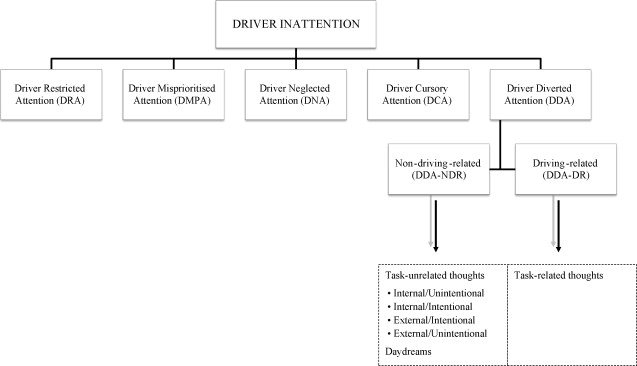
\includegraphics[width=\textwidth]{driver_inattention_taxonomy} 
	\caption{Taxonomy of driver inattention. Reproduced AS-IS with permission from \citep{reganDriverDistractionDriver2011}}
	\label{fig:taxonomy_inattention}
\end{figure}
\todo{REPRODUCE FIGURE, REMOVE DASHED BOXES}

\paragraph{\gls{dra}} inattention caused by biological factors (e.g. fatigue) and therefore can be monitored.

\paragraph{\gls{dmpa}} incorrectly paying too much attention to one area of the driving task at the expense of a second equally or more important task. Probably can't be monitored but the consequences can be mitigated through \gls{adas} systems such as automatic emergency braking or blind-spot warnings

\paragraph{\gls{dna}}  \todo{Need to actually include this bit...}

\paragraph{\gls{dca}} cursory attention to elements of the driver task, for example a quick glance in the rear-view mirror without fully processing the scene. Probably can't be monitored but the consequences can be mitigated through \gls{adas} systems such as automatic emergency braking or blind-spot warnings

\paragraph{\gls{dda}} `The diversion of attention away from activities critical for safe driving towards a competing activity' \citep{reganDriverDistractionDriver2011}. This category encompasses driver distractions, which can be considered to be manual, visual, cognitive, or a combination of the above, in nature.

Some of these definitions are nuanced, and the authors themselves acknowledge that it is unlikely to be able to distinguish between some of the categories in practice. However the key points that are relevant to this work are that driver inattention can fall into a number of categories, with \gls{dra} and \gls{dda} being most relevant for a driver attentiveness monitoring system.

\gls{dra} and some of the \gls{dda} causes of inattention could be monitored by a driver attentiveness monitoring system, and this directs the remainder of this work.  

Looking at \gls{dda} in more detail, driver distraction can be classified as one or more of the following categories:
\todo{find a reference for this?}
\begin{itemize}
	\item Visual distraction, where the driver's visual focus is a non-driving related subject, such as a mobile phone screen or a passenger.
	\item Manual distraction, where a driver's feet or hands are removed from the pedals or steering wheel respectively.
	\item Cognitive distraction, where a driver's thoughts are focussed on a task not related to the driving task, such as an involved conversation with a passenger.
\end{itemize}


\subsubsection{Automated driving systems}
\todo{Should be ok as first draft}
As \glspl{ads} become more common and more advanced, the issue of driver inattention is likely to become even more critical. One particular area of concern is partially-autonomous vehicles, where the driver is still required to monitor and react to the environment while the \gls{ads} is performing certain driving tasks.  In \citep{J3016_201806} SAE International introduced a taxonomy and definitions for six levels of driving automation which is widely used in the discussion of autonomous vehicles. A summary of the six levels is shown in \cref{fig:av_levels}. These six levels of autonomy are based on four main factors which differentiate between whether the (human) driver or the automated system is responsible for certain tasks: 

\begin{enumerate}
	\item Who is performing primary driving actions (lateral and longitudinal control) 
	\item Who is detecting and responding to obstacles and events
	\item Who is the fallback should the automated system fail or reach an area outside of its operational design domain
	\item The extent and any limitations on the operational design domain\textemdash the environment(s) in which the automated system is designed to operate
\end{enumerate}

\begin{figure} 
	\centering
	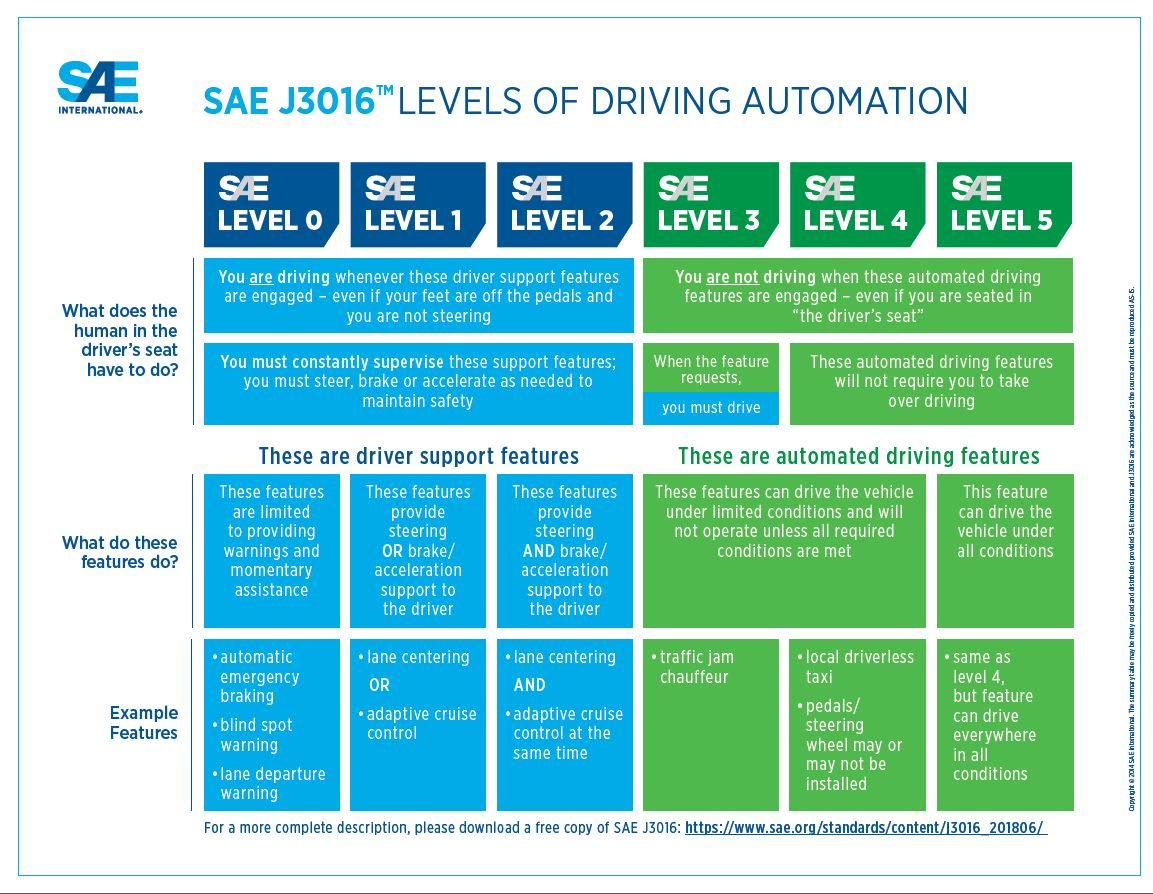
\includegraphics[width= 0.95\textwidth]{sae_av_levels} 
	\caption{Levels of driving automation. Reproduced AS-IS with permission from \citet{J3016_201806}}
	\label{fig:av_levels}
\end{figure}

A brief discussion of these levels of driving automation follows, highlighting the importance of driver attentiveness monitoring at the different levels of automation. 

SAE level 0 systems feature no driving automation. The human driver is always controlling the lateral (steering) and longitudinal (acceleration and braking) motion of the vehicle, and detecting and responding to obstacles and events during the driving task. There are exceptions for \gls{adas} such as automatic emergency braking, but these are not considered further here as they do not relate to the issue of driver attentiveness. Driver inattention and distraction is a concern in level 0 systems, with a review reporting driver inattention or distraction as a cause in approximately one quarter of \glspl{rtc} in the United States \citep{youngDriverDistraction2007}. A system with the capability to detect inattention or distraction could provide the driver with visual, audible or tactile alerts and warnings may increase driver attention or cause the driver to take a rest stop, and so reduce the likelihood of an \gls{rtc}.

In SAE levels 1 and 2 the human driver of the vehicle is always considered to be driving the vehicle, even if lateral and/or longitudinal control (steering and/or braking) is performed by the \gls{ads}. A level 1 system provides steering \emph{or} accelerator and brake support to the human driver, while a level 2 system can perform both tasks. The Tesla vehicles involved in the \glspl{rtc} in \cref{sec:motive} were SAE level 2 vehicles with the Tesla \gls{ads} system, `Autopilot' engaged. 

An SAE level 3 autonomous vehicle is capable of driving the vehicle under limited conditions, and the human is not considered to be the driver while the level 3 \gls{ads} is engaged. However the human driver must take back control of the driving task when requested to do so by the \gls{ads}. It is hopefully apparent that there are significant concerns and issues around driver distraction and inattention in level 1, 2 and 3 \gls{ads}, and these are areas where a low cost driver attentiveness monitoring system will offer benefits in safety and ....  \citet{teohWhatNameDrivers2020} report drivers consider many actions to be safe while a level 2 system is in operation, they're wrong, particularly bad for Autopilot. Prompt to remind drivers to pay attention, or disable the system where necessary etc...

\citet{goncalvesDrowsinessConditionalAutomation2016} experimentally investigated passive fatigue caused by underloading a driver when autonomous systems are used. The majority of subjects reported high levels of drowsiness within 15 minutes, and a decrease in performance when responding to take over requests was found.

Levels 4 and 5 can both be considered fully autonomous and the human driver is never expected or required to take control of the driving task. Level 4 is restricted to operate in limited circumstances, while level 5 automation can drive under all conditions. Driver attentiveness monitoring is not directly relevant to level 4 and 5 systems, however the closely related task of driver mood monitoring may be beneficial, allowing the \gls{ads} to tailor the vehicle ambience, driving route and style to the human occupants' current mood.

In addition to all of this, a driver monitoring system which includes monitoring of vital signs may provide valuable information to emergency response and accident investigation teams (driver is alive but deteriorating, driver was healthy before \gls{rtc} vs driver had heart attack before \gls{rtc}). 



\subsection{Approaches for monitoring inattention} \label{ssec:approaches}
\todo{tie all of this together, need to decide on structure... strucutre based on measure?}
%
%\paragraph{notes}
%Present existing methods, categorise as:
%\begin{itemize}
%	\item Driving behaviour measures:
%	\begin{itemize}
%		\item Driving input measures (steering, brakes, accelerator)
%		\item Lane-keeping
%		\item Spacing to surrounding vehicles
%	\end{itemize}
%	\item Driver physiological measures:
%	\begin{itemize}
%		\item Heart rate
%		\item Eye motion tracking
%		\item Vision based systems
%		\item Head motion tracking
%		\item Facial expressions
%	\end{itemize}
%	\item Discuss methods which combine measures
%	\item Driver models (Kalman Filter of the driver?)
%\end{itemize}
%
%\paragraph{content}
A number of approaches for driver attentiveness monitoring have been proposed in the literature, using a variety of measured signals to detect the different forms of driver inattention, \gls{dra} and \gls{dda}, introduced previously. Due to the different causes and symptoms of \gls{dra} and \gls{dda} some approaches are better suited to detecting one or the other. Monitoring approaches can either be categorised according to the form(s) of driver inattention they are best suited to monitoring or according the measures that are used to assess attentiveness. This section considers the relevant literature, starting with those that investigate \gls{dda} detection before considering \gls{dra} monitoring and works that monitor both forms of driver inattention.

\todo{decide what to do with this}
is identified and discussed according to the measures used, as this is more useful because..... A taxonomy for all the measures considered in this work is shown in \cref{fig:taxonomy_measures}

\begin{figure} 
	\centering
	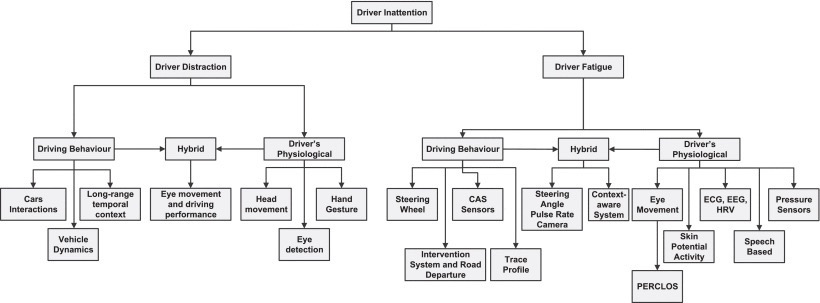
\includegraphics[width=\textwidth]{inattention_inputs_taxonomy} 
	\caption{Taxonomy of driver inattention measures \citep{koesdwiadyRecentTrendsDriver2017}}
	\label{fig:taxonomy_measures}
\end{figure}
\todo{REPRODUCE FIGURE TO REFLECT CONTENTS OF THIS WORK}
\todo{Present summary diagram similar to fig. 3 of \citep{koesdwiadyRecentTrendsDriver2017}}

\subsubsection{Driver Distracted Attention monitoring}

Works in this category aim to detect driver distractions, which can be considered to be visual, manual, cognitive, or a combination of the above, in nature. 

\paragraph{\citet{wollmerOnlineDriverDistraction2011}} Uses \gls{lstm} \glspl{rnn} for the classification of driver distraction with 96.6~\% accuracy. Measures are head tracking and driving behaviour signals: steering wheel angle, throttle position, speed, heading angle, lateral deviation.  Distraction is classified using either two, three or six classes to investigate the possible granularity of the classification approach. Training and testing used a real world driving dataset. Distraction tasks were non-driving related operation of in-vehicle information systems such as a radio and satellite navigation system. This type of task involves visual, manual, and cognitive distractions. The authors test the use of low level signals and statistical functions of the signals over a number of frames (\emph{functionals}), finding that the use of functionals as an input to the \gls{lstm} results in greater accuracy, although using low level input signals still outperformed \gls{rnn} and \gls{svm} based implementations.

Using the \gls{lstm} is good because time series data... need to make this point better... 

Note that the driving behaviour signals used in this work are less relevant for level 2 and 3 automated vehiclesm as lateral and longitudinal control is by the \gls{ads} and not the human driver.

\paragraph{\citet{liangHybridBayesianNetwork2014}} use a layered algorithm with \gls{dbn} and supervised clustering to detect cognitive distraction from eye movements and driving behaviour. Driving behaviour is measured as the standard deviation of both steering wheel angle and lane position, as well as steering error. Steering error is a metric of steering smoothness proposed by the authors, calculated by comparing the steering wheel angle to a steering angle predicted by a second-order Taylor expansion. Supervised clustering is used in the lower layer of the algorithm to identify key features and represent them in an abstract fashion, improving the computation speeds of the \gls{dbn} layer.  Data from a simulator with auditory cognitive distraction was used to train the layered layered algorithm, with \gls{dbn} and \gls{svm} algorithms trained on the same data for comparison. \gls{dbn} algorithms have the benefit of being more interpretable than \glspl{svm}, but at the cost of greater computational complexity. The layered algorithm performed comparably to the benchmark methods in detecting distraction, but with reduced training and prediction times compared to the \gls{dbn} and improved interpretability compared to the \gls{svm}. 

Again the driving behaviours are not applicable to level 2 and 3 autonomous vehicles.

\paragraph{\citet{aksjonovDetectionEvaluationDriver2019}} Rule based expert system using fuzzy logic for measuring driver distraction. Tested via driver-in-the-loop experiments in a simulator, where the driver completes a distracting task while driving (replying to a text message). Measures relate to driving performance. Nonlinear regression is used to output a single number as a measure of distraction, a distinction from many works which instead classify levels of distraction. An \gls{ann} is trained to predict the lane keeping and speed deviation based on speed limits and turn radius. This is compared to actual lane offset and speed deviations with a fuzzy logic control returning a percentage measure of driver distraction. The prediction model requires the driver to first drive the route as accurately as possible which presents an issue for generalisation to new environments. The resulting measurements of driver distraction align with the periods in which the drivers were performing the distraction task, although it is not apparent that a numerical measure of distraction is any more valuable than a suitable classification scale. Once more, the use of driving behaviours means this approach will be of limited value in level 2 and 3 vehicles.

 \paragraph{\citet{dingInattentiveDrivingBehavior2019}} \gls{fmcw} radar used to detect driver movements for inattention detection. Potentially more acceptable to consumers as does not require a camera. Seven driver behaviours were investigated with time-Doppler spectrograms and range-Doppler trajectories measured by \gls{fmcw} radar. Frequencies investigated are 5.8 and 24~Ghz, with the 5.8~Ghz radar resolution found to be too low for accurate results. Testing is performed on six human subjects.
 
 Radar signals were processed to e...
 
 A range of machine learning methods were tested to classify the driver attentiveness based on features extracted from the time-Doppler spectrogram and range-Doppler trajectory. A Bagged Trees classifier was found to have the highest average accuracy across the seven investigated driver behaviours, achieving 94.8\%, 93.3\% and 95.6\% average accuracy for time-Doppler, range-Doppler, and combined feature inputs respectively. 
 
 \todo{This is an interesting work, expand on it}
 
\subsubsection{Driver Restricted Attention}
The works considered here aim to monitor \gls{dra}, primarily categorising it in the form of fatigue or drowsiness.
 
 \paragraph{\citet{jungDriverFatigueDrowsiness2014}} Electrocardigram (ECG) sensor embedded in steering wheel. Sample ECG signals at 100 Hz. Driver state assessed by evaluating heart rate variability (HRV), the variation of the time interval between heart beats. HRV can be used to evaluate the autonomic nervous system (ANS) status and can indicate normal, fatigued and drowsy states. HRV analysis methods can be in the time domain or the frequency domain. Time domain HRV is based on beat-to-beat intervals, frequency based HRV is by measuring the power spectral density (PSD) using parametric fast Fourier transforms.
 
 Testing of the system is limited, with only two test subjects over a two hour driving test, and results are reported qualitatively. More robust testing and reporting would be required before such a system was used in production. Additionally, the signal is measured using contact based sensors, requiring the driver to have their hands correctly positioned on the wheel. 
 
\paragraph{\citet{zhangAutomatedDetectionDriver2014}} Various entropy and complexity measures applied to simultaneously recorded \gls{eeg}, \gls{emg} and \gls{eog} signals for real-time detection of fatigue. An \gls{ann} is trained to classify fatigue in one of four levels using the complexity measures. Accuracy of estimation between 96.5\% and 99.5\%. Obvious weakness is that \gls{eeg}, \gls{emg} and \gls{eog} signals are contact-based measurements using complex and expensive equipment (electrodes placed on occiput, eyelids, and neck). \todo{Probably a good reference but could do with understanding it better?}

\paragraph{\citet{tsuchiyaHeartbeatDetectionTechnology2020}} 24GHz microwave Doppler radar based heart rate detection. Sensor is placed in seat back to avoid interference from arm motions  Vibrations (e.g. from driving) cause noise to be superimposed over the sensor signal reducing the SNR (signal to noise ratio). The authors introduce an algorithm to cope with this. 

Electrodes on steering wheels don't work if driver's hands are not on the wheel or the sensor, camera based systems raise concerns of intrusion / privacy. 

Electrocardiogram: peaks of electrical activity are called P,Q,R,S, and T-waves. Interval between two consecutive R peaks is heartbeat interval (R-R interval, RRI). A heartbeat generates a small displacement of the body surface which is detected by radar system. However  respiration and body movements fal in the same band, making it difficult to extract heartbeat.

Experimental evaluation via in-car testing with ECG as reference sensor. Improved accuracy during driving compared to previous method but still poor equivalence to ECG reference sensor.

\paragraph{\citet{liDetectionDriverDrowsiness2013}} wavelet transform of \gls{hrv} signals measured using \gls{ppg} with a \gls{svm} classifier with categories alert and drowsy. Incorporated into an application which will find a nearby rest location if fatigue is detected. A $1^\text{st}$ order differential operation is used to filter movement induced noise from the  \gls{hrv} time series data, which is then decomposed into nine wavelet levels before an \gls{svm} is used to classify the level of fatigue. The system was tested with four participants in a driving simulator. The accuracy of the classification of the drivers' fatigue (as alert of drowsy) was 95\%.

\paragraph{\citet{yuDriverDrowsinessDetection2019}} System uses four models to detect fatigue: representation learning, scene understanding, feature fusion, and fatigue detection. The representation learning model uses a 3D \gls{cnn} that allows for a sequence of frames to be used as an input to the \gls{cnn}, and outputs a spatio-temporal representation of the scene. This representation is passed through a scene understanding model which interprets key features of the scene, including illumination and head, mouth and eye conditions. The output of the scene understanding model is combined with the scene representation in a fusion model, before a detection model classifies the driver as fatigued or alert. The combined model is resilient to variations in scene composition, such as the wearing or removal of glasses, and variation in light conditions. 
 
The system was trained and tested using the \gls{nthu} Drowsy Driver Detection video dataset \citep{wengDriverDrowsinessDetection2017} which consists of over nine hours of video data of 36 subjects performing simulated driving tasks while making various facial expressions in response to external requests. A potential issue with this dataset is that the facial expressions and other displays of fatigue are being simulated by the participants by them acting as if they were fatigued. It is likely that the facial expressions and behaviour of an individual experiences real fatigue will differ from these simulated expressions. However this dataset does allow researchers to demonstrate the feasibility of a given approach, even if further training and testing is required in real-world conditions.

The average classification accuracy was 76.2\% and was consistently more accurate than alternative approaches tested on the same dataset. Although the final accuracy reported is low compared to some other methods considered here, it is difficult to directly compare works which are assessed under different conditions and using different datasets. In addition the dataset used in this work includes a number of challenging scenarios, such as direct sunlight, night and the wearing and removal of glasses.

\paragraph{\citet{gaoEEGBasedSpatioTemporal2019}} Also using a 3D \gls{cnn} but with \gls{eeg} as input. Result is a \gls{eeg} based spatio-temporal \gls{cnn} to detect driver fatigue. Three convolutional layers were used Data for training and testing is from a driving simulator with eight subjects. Two class classification accuracy was 97.37\%, higher than all eight comparison methods considered by the authors.

\paragraph{\citet{crayeMultiModalDriverFatigue2016}} Multi-modal - used audio, color video, depth map, heart rate, and steering wheel and pedal positions. Able to detect both fatigue and distraction, with 98.4\% and 90.5\% accuracy respectively. Input signals are processed by three modules (vision, audio, other) with each module producing an independent estimation of driver fatigue and distraction using \glspl{hmm}. The outputs of each module are fused with contextual information and a Bayesian network. System separately processes driver fatigue and distraction, and detects the type of action the driver is performing to estimate driver distraction.  Three modules: 
\begin{itemize}
	\item Vision module processes arm position, face orientation, facial expression and eye movements.
	\item Voice module process audio signals.
	\item Other signals module processes heart rate, and steering wheel and pedal positions.
\end{itemize}
Modules are independently processed and can be enable or disabled individually. Dataset is temporal so \glspl{hmm} are used. Two separate Bayesian networks are used, one each to detect fatigue and distraction.

Driving simulator based. Dataset for training and testing gathered from eight subjects. Drivers simulated the symptoms of fatigue (yawning, closing their eyes) Drivers were also tasked with completing a number of distracting tasks during the experiment. Distraction was classified as one of either two or five classes, with the two class classification being more accurate. Driver arm position was found to be the most accurate indicator of distraction, with eye behaviour is being the lowest accuracy indicator, highlighting the importance of fusing multiple signals to get an accurate classification. 

\paragraph{\citet{duaAutoRateHowAttentive2019}}  A five rating scale of driver attentiveness based on \gls{cnn} and \gls{gru} for spatio-temporal representation of visual sensory input, using the front facing camera of a windscreen mounted smartphone. Dataset of 2900 unique video segments, each 10~seconds long, covering 30 drivers performing real-world driving tasks in a large city. Each video segment was rated on a five point scale by human annotators. 

A number of pre-trained \glspl{cnn} are used to extract both generic features and specific facial features from the input frames. The outputs of both the generic and specific networks are combined using \glspl{lstm} so taht the temporal nature of both fatigue and distraction are considered. The system was tested on 782 unseen videos with an accuracy of 70\% compared to the human annotators.

\paragraph{\citet{fuDynamicDriverFatigue2016}} \gls{hmm} applied to biological signals for fatigue detection. Measures are \gls{eeg}, \gls{emg} and respiration. Tested during real-world driving on 12 professional driver. Drivers self-reported their state as alert, mildly fatigued or fatigued. Measured signals were processed as follows. A \gls{fft} and Butterworth band-pass filters were applied to the \gls{eeg} signal to get the power spectrum of three fatigue related frequency bands, theta, alpha and beta. \todo{probably need more here....}



\paragraph{\citet{zhouPredictingDriverFatigue2021}} Explainable fatigue prediction using XGBoost prediction model and SHAP for explainability.  Experiments performed in a driving simulator, with the subject performing a simple driving task before an \gls{ads} took over the driving task, with the subject supervising the \gls{ads} system but completing no additional tasks, with the intention of inducing passive fatigue as discussed by \citep{goncalvesDrowsinessConditionalAutomation2016}. \gls{perclos} was used as the ground truth signal for fatigue. Measures used for the prediction model were related to heart rate and respiratory rate, as well as \gls{ecg}, steering wheel torque and angle, and driver posture. The most important measures according to SHAP value were \gls{hr} (averaged over 60 seconds), \gls{hrv} and breathing rate (averaged over 60 seconds). Interesting \gls{ecg} was reported as the second lowest important measure - \gls{ecg} is commonly used for fatigue detection.  
	

%\paragraph{\citep{koesdwiadyRecentTrendsDriver2017}} A high-level survey of driver monitoring systems. It doesn't seem great but probably provides some good references to follow up on. Discusses types of driver inattention which is useful. Introduces a taxonomy of driver distraction monitoring sources which is probably worth exploring. Main sources of driver distraction detection:
%\begin{itemize}
%	\item Driving behaviour measures, including LSTM tracking head movement \citep{wollmerOnlineDriverDistraction2011}
%	\item Physiological measures of driver (all vision based in this paper)
%	\item Hybrid methods (driving behaviour and physiological measures)
%\end{itemize}
%
%Use of Dynamic Bayesian Networks to detect distraction via driving behaviour and eye movement \citep{liangHybridBayesianNetwork2014}
%
%Main sources of driver fatigue detection:
%\begin{itemize}
%	\item Driving behaviour measures
%	\item Physiological measures:
%	\begin{itemize}
%		\item Eye and face movement
%		\item Speech
%		\item PERCLOS (percent of eye closure)
%		\item Skin \citep{kurianDrowsinessDetectionUsing2014a}
%		\item Biological signals \citep{zhangAutomatedDetectionDriver2014}
%	\end{itemize}
%\end{itemize}
%
%\paragraph{\citep{reganDriverDistractionDriver2011}} Introduces definitions and taxonomy for driver distraction and driver inattention (distinguishing between the two).
%
%Driver inattention is defined as `insufficient, or no attention, to activities critical for safe driving'. This is a good reference with good taxonomy etc.
%
%
%\paragraph{\citep{sikanderDriverFatigueDetection2019}} Fatigue detection methods are implemented as either: bio-mathematical models, rule based, or machine learning models. Remember that fatigue is only one of the causes of driver inattention.  A good reference and source of references for fatigue related approaches.
%
%\begin{itemize}
%	\item Bio-mathematical models are more relevant for workload management tasks (aircrew rotas, driver schedules etc.)
%	\item Rule based models (like expert systems) include Fuzzy Inference Systems, e.g. \citep{aksjonovDetectionEvaluationDriver2019}
%	\item Machine learning based implementations such as Artificial Neural Networks (ANN) or Support Vector Machines (SVM). Lots of references to consider....
%	\begin{itemize}
%		\item \citet{liDetectionDriverDrowsiness2013} use SVM classifier on PPG (photoplethysmography) derived HRV (heart rate variability)
%		\item Vision based CNN approaches \citep{yuDriverDrowsinessDetection2019} and EEG based CNN approaches \citep{gaoEEGBasedSpatioTemporal2019}
%	\end{itemize}
%\end{itemize}
%
%Figure 2 in Section \textsc{V} is a very good way of representing / summarising the approaches taken in previous works.
%
%Separate methods from input sources.  Method exanples are:
%\begin{itemize}
%	\item Bio-mathematical
%	\item Rule based
%	\item Machine learning
%\end{itemize}
%
%Example signal sources are:
%\begin{itemize}
%	\item Driving behaviours (steering behaviour, lane keeping, driving time)
%	\item Driver physiological measures (heart signal, brain signal, PERCLOS, eye tracking, posture)
%	\item Hybrids
%\end{itemize}




\subsection{Analysis} \label{ssec:analysis}

\paragraph{notes}
Summary table 
Summary graph
Discuss

\cref{fig:summary} driver physiological measures are mostly used for \gls{dra} type inattention such as fatigue, while driving and driver behaviour measures are predominately used to detect driver distraction.

This presents an issue as driving behaviour measures are likely to be meaningless in level 2 and 3 autonomous vehicles, where lateral and longitudinal control is by the \gls{ads} for long periods of time. 

Many of the driver physiological measures proposed involve contact based sensors which is not likely to be accepted by consumers. In addition these sensors are expensive and require careful positioning.

\begin{figure} 
	\centering
	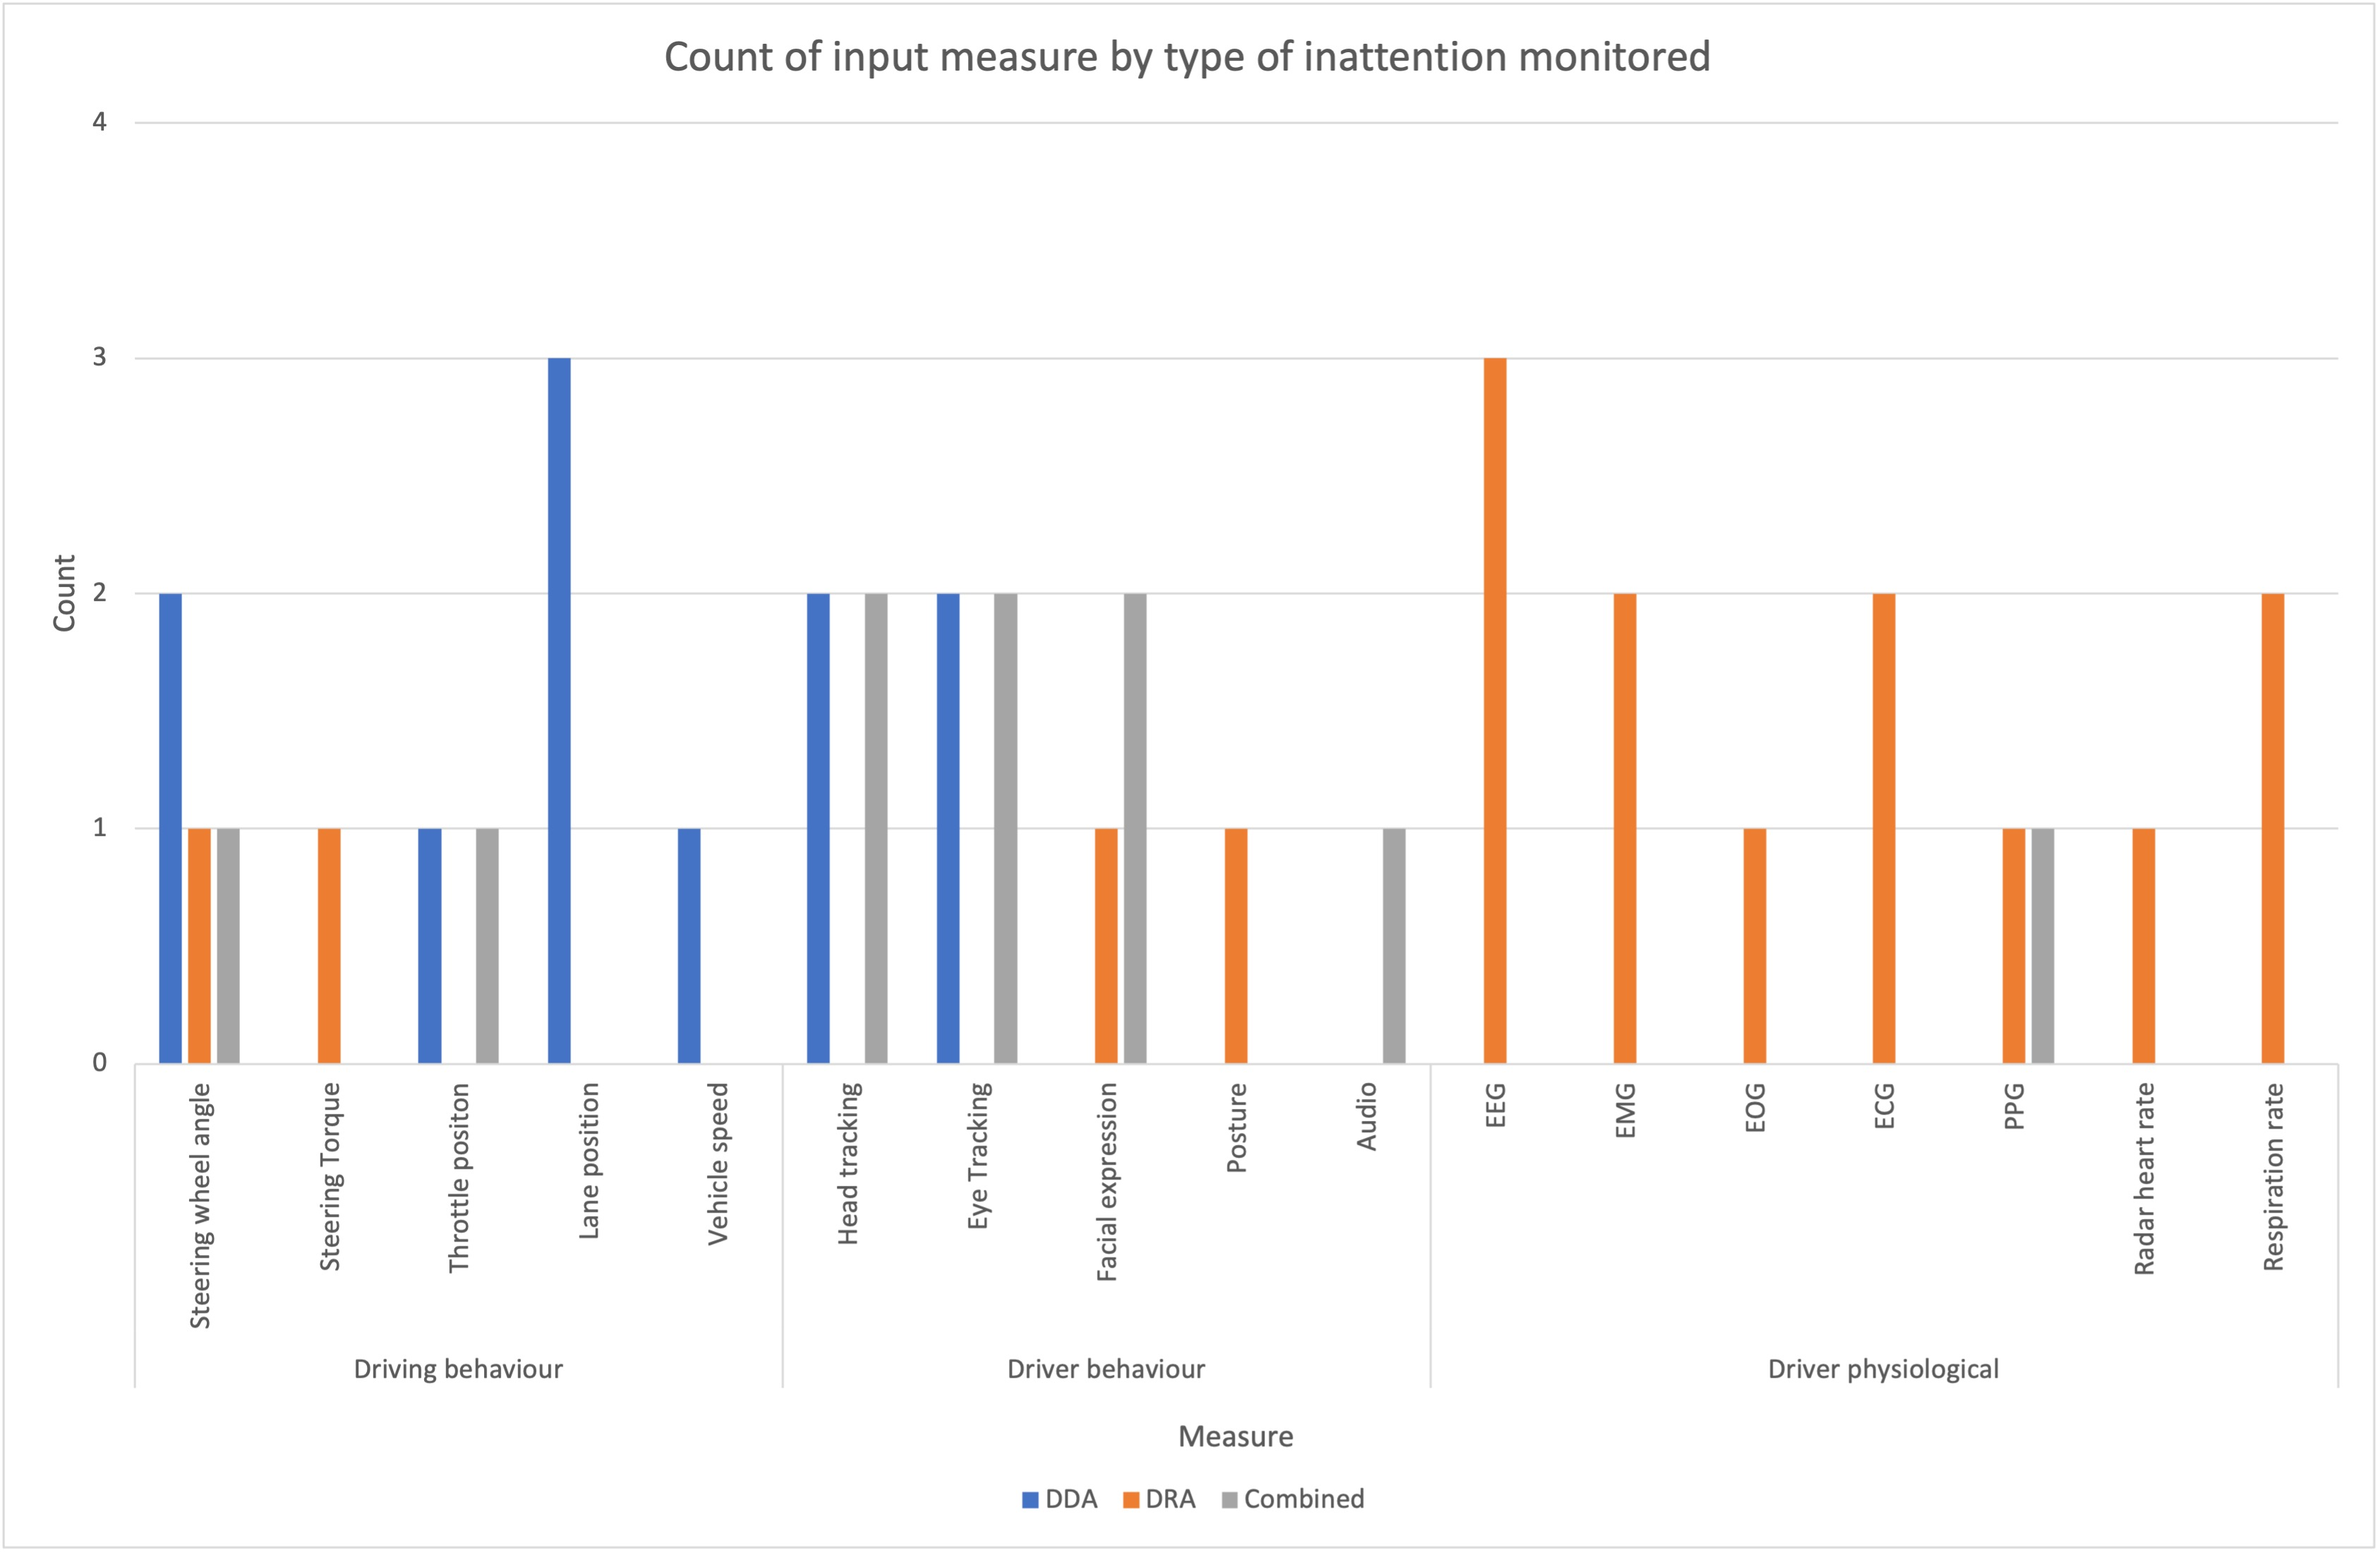
\includegraphics[width=0.95\textwidth]{summary_graph} 
	\caption{A summary of measurement inputs identified in this review, categorised by the type of driver inattention detected in the work.}
	\label{fig:summary}
\end{figure}

%\paragraph{notes}
%Use preceding sub-section as input to discuss:
%\begin{itemize}
%	\item Trends
%	\item Weaknesses
%	\item Gaps
%	\item Issues
%\end{itemize}
%
%\paragraph{content}
% 


\section{Non-contact vital sign monitoring} \label{sec:vital_sign}
%\glsresetall
\todo{better introduction}
%\paragraph{notes}
%Discuss vital sign monitoring in a healthcare setting (personal and clinical), with a view to potential cross-overs between driver distraction and inattention monitoring and vital sign monitoring (in both directions).
%
%\paragraph{content}

Many of the driver inattention detection methods discussed in \cref{ssec:approaches} use driver vital signs as an input. The acquisition of driver vital signs poses a number of challenges, including the expense and complexity of the sensing equipment, and the discomfort and distraction caused by contact-based sensors. These challenges also exist in healthcare settings, and so a significant body of work investigates \gls{ncvs} monitoring devices in a clinical setting. This section considers existing literature which make use of vision and radar inputs as these align with the automotive setting.

%\subsection{Vital signs} \label{ssec:vital_signs}
%
%\paragraph{notes}
%
%Briefly introduce and define the key vital signs used in healthcare settings (`textbook' definitions)
%\begin{itemize}
%	\item \gls{hr} commonly measured using \gls{ecg}
%	\item \gls{rr}
%	\item \gls{spo2} commonly measured using an pulse oximeter
%\end{itemize}

%\subsection{Non-contact vital sign monitoring}

%\paragraph{notes}
%Brief overview of existing vital sign monitoring approaches:
%\begin{itemize}
%	\item Contact based (very brief)
%	\item Non-contact based (focus)
%	\begin{itemize}
%		\item Vision based
%		\item Radar based
%		\item Other?
%	\end{itemize}
%\end{itemize}

\subsection{Radar}
\paragraph{notes}
The original paper on non-invasive microwave measurement of respiration is  \citep{linNoninvasiveMicrowaveMeasurement1975} (for respiration).  Radar based vital sign monitoring relies on measuring the Doppler shift of the radar signal which is caused by movement of the chest wall from breathing and heart pumping. Number of different frequencies have been assessed \cref{fig:radar_freqs}. Majority of work focussed on 24~Ghz but the \gls{uwb} at 24~Ghz is being phased out and will not be available after January 1, 2022 \citep{ramasubramanianMovingLegacy242018}. 

The original paper on non-invasive microwave measurement of respiration is  \citep{linNoninvasiveMicrowaveMeasurement1975}. The basic principle of measurement is based on Doppler shift caused by movement of the subject's chest wall.  Two most commonly used radar topologies are \gls{cw} (including \gls{fmcw}) and \gls{uwb}. Advantages and disadvantages are discussed in the paper (probably good to include). Table 1 in particular is a nice summary. Discusses radar front end architectures - heterodyne vs homodyne, single vs quadrature channel.

Increasing frequency reduces wavelength and increases the sensitivity to small displacements. mmWave region corresponds to frequencies between 30~GHz to 300~GHz.  Higher frequencies have numerous advantages:
\begin{itemize}
	\item Improved range resolution
	\item Reduced device form factor
	\item Improved directionality and therefore increased range
\end{itemize}

\begin{figure} 
	\centering
	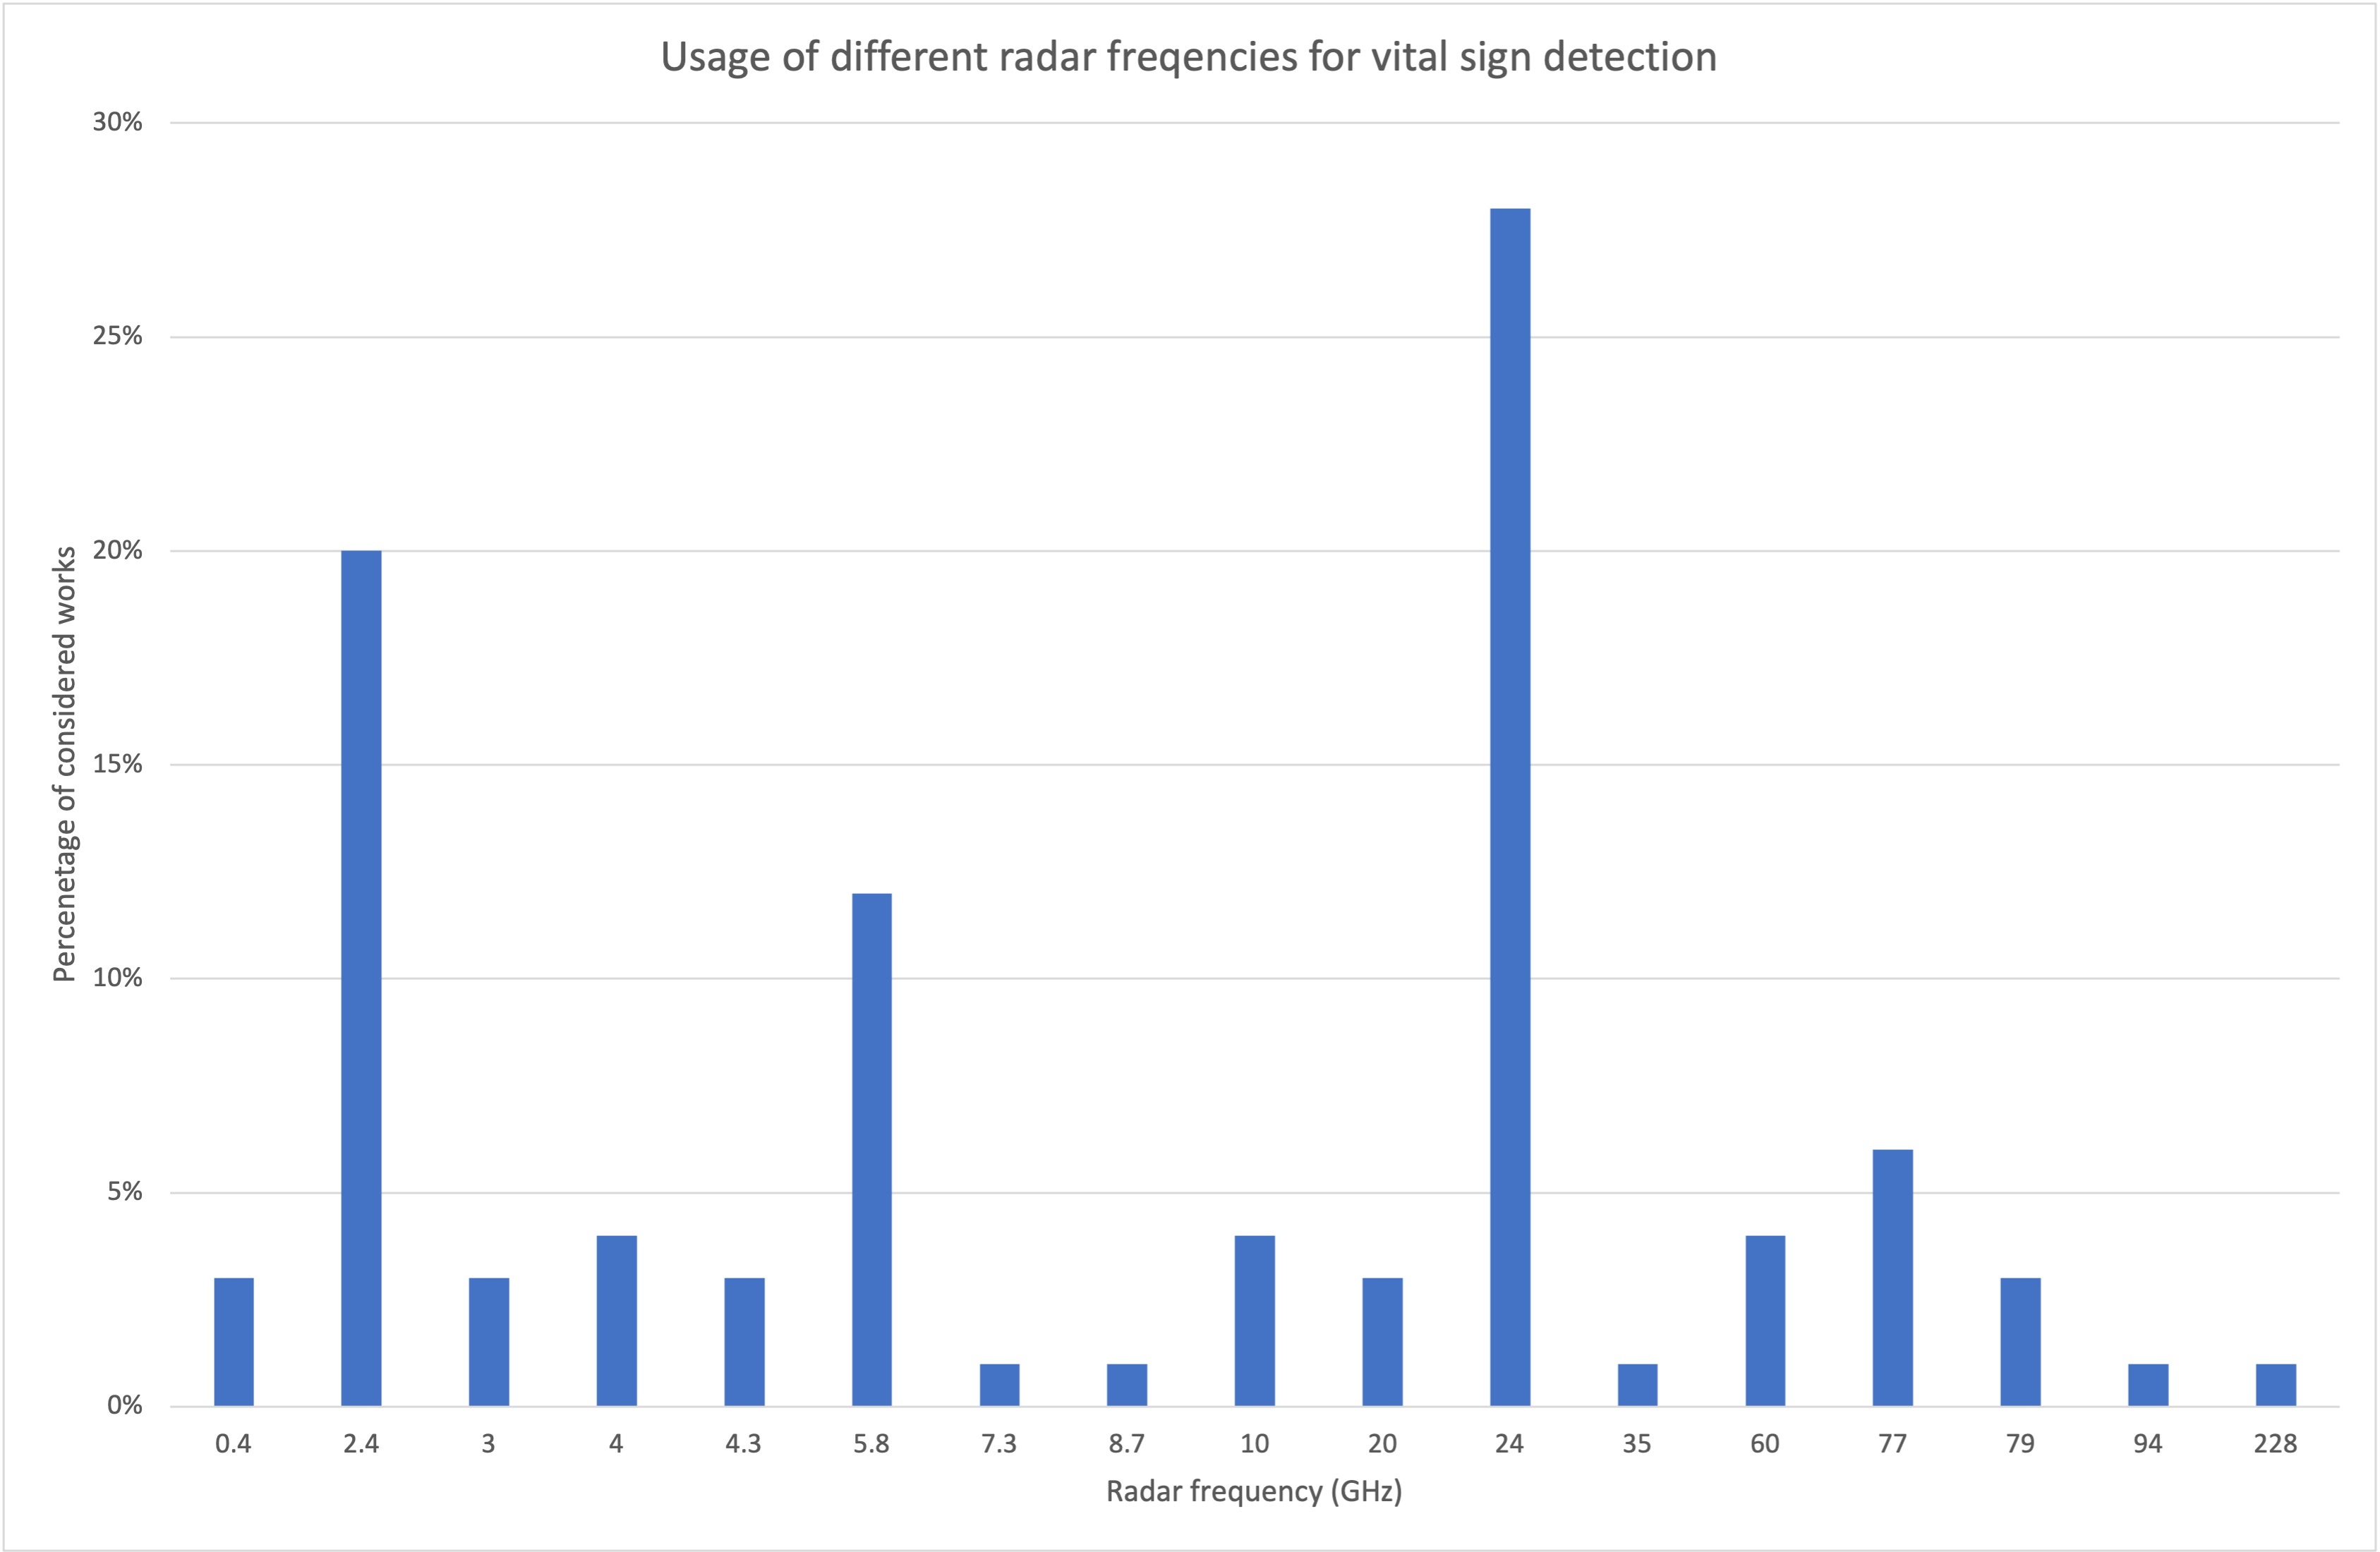
\includegraphics[width=0.95\textwidth]{radar_frequencies} 
	\caption{A summary of the radar frequencies used in a variety of works. Data sourced from \citet{singhMultiResidentNonContactVital2021}}
	\label{fig:radar_freqs}
\end{figure}

\paragraph{\citet{willAdvancedTemplateMatching2017}} use a 24~Ghz \gls{cw} radar with an advanced template matching algorithm for instantaneous heartbeat detection. Five different types of heartbeat signal templates are used, each defined by six features. When comparing the interbeat interval to a reference \gls{ecg} signal the \gls{rmse} was 18.0~ms, compared to 68.2~ms with a previous template matching approach.

\paragraph{\citet{willRadarBasedHeartSound2018}} detect heart sounds using an unmodulated continuous wave radar and a hidden semi-Markov model. \gls{ecg}and \gls{pcg} measurements are used as ground truth for heartbeat and heart sound detection respectively. Heart sounds detected using this method were strongly correlated to heartbeats measured using \gls{ecg}, with an F-score of $92.22\pm 2.07 \%$.

\subsection{Vision}
Vision based monitoring systems are based on \gls{rppg}, which uses a camera to measure the changes in blood volume in blood vessels under the skin. \citet{verkruysseRemotePlethysmographicImaging2008} were the first to demonstrate that \gls{ppg} signals can be acquired remotely under ambient lighting conditions using a consumer grade camera pointed at the subject's face. The patients face and a background \gls{roi} are identified. Pixel values in each color channel are spatially averaged to improve \gls{snr} at the expense of spatial resolution. 

Motion artefacts are identified as disrupting readings. Green channel shows best signal for \gls{hr} detection.

{\citet{tarassenkoNoncontactVideobasedVital2014} extended on the above work, incorporating an auto-regressive model to filter out noise caused by artificial light flicker. 

\citet{villarroelContinuousNoncontactVital2014} look at neonatal intensive care setting, using the same techniques described above to monitor \gls{hr}, \gls{rr}, and \gls{spo2}. Infants in incubators. Subjects were 30 pre-term infants. Found large changes in the ambient light conditions, subject movement and no visible skin as issues with the method. Reported that, for an absolute error of 4~\gls{bpm}, there was no significant difference in the measurement differences for the vision based method and the \gls{ppg} or \gls{ecg} methods, when compared to the differences between the \gls{ppg} and \gls{ecg} measures themselves.

\citet{villarroelNonContactVitalSign2017} use a video camera to estimate heart rate, respiratory rate and changes in peripheral oxygen saturation in a real-world healthcare setting (patients undergoing dialysis). Two \gls{ppg} sensors are used at to different locations on the subject as a reference signal for \gls{hr} and \gls{spo2}. \gls{ecg} and a chest belt were used for \gls{rr} reference signals. System tested over 61 dialysis sessions, a total of 219.8 hours of video. The mean absolute error of the \gls{hr}, \gls{rr} and \gls{spo2} estimations were 2.8~\gls{bpm}, 2.1~\gls{bpm} and 2.5\% respectively. Note that the errors between the two reference pulse oximeters were 1.87~\gls{bpm} and 0.97\% for \gls{hr} and \gls{spo2} respectively, which is comparable to the errors in the estimated signals.  A problem with this approach is that a large number of the video sessions recorded were not suitable as inputs due to patient and camera movements, obstructed views of the patients face and medical interventions. Also doesn't work in low light.

This technology is being commercialised by Lifelight \citep{suzanneLifelightXimLimited} and a number of clinical trials have been completed or are in progress. 


%
%\paragraph{\citep{singhMultiResidentNonContactVital2021}} Review paper of multi-resident non-contact vital sign monitoring using radar.
%
%Applications in health care including infant monitoring, telehealth, sleep monitoring, skin allergies and burn cases.  Different none contact methods include:
%\begin{itemize}
%	\item Optical vibro-cardigraphy
%	\item audio
%	\item thermal imaging
%	\item RGB camera
%	\item ultrasound radar2
%	\item microwave radar
%\end{itemize}
%
%Figure 2 in the paper gives a simple representation of a doppler radar based system. The original paper on noninvasive microwave measurement of respiration is  \citep{linNoninvasiveMicrowaveMeasurement1975}. The basic principle of measurement is based on Doppler shift caused by movement of the subject's chest wall.  Two most commonly used radar topologies are \gls{cw} (including \gls{fmcw}) and \gls{uwb}. Advantages and disadvantages are discussed in the paper (probably good to include). Table 1 in particular is a nice summary. Discusses radar front end architectures - heterodyne vs homodyne, single vs quadrature channel.
%
%Section D gives a good overview of how radar \gls{ncvs} works. One way to increase SNR is by increasing transmission power but there are limits as this can lead to damage to tissue / harm to health etc. FInd a source for guidelines / standards / regulations / legislation?
%
%Increasing frequency reduces wavelength and increases the sensitivity to small displacements. mmWave region corresponds to frequencies between 30~GHz to 300~GHz.  Higher frequencies have numerous advantages:
%\begin{itemize}
%	\item Improved range resolution
%	\item Reduced device form factor
%	\item Improved directionality and therefore increased range
%\end{itemize}
%
%Is attenuation an issue around the 60 GHz range?
%
%Figure 5 gives an excellent view of the frequencies investigated for \gls{ncvs} in previous works



\section{Gaps and opportunities}

Many works tested in driving simulators only and with low number of subjects

Many approaches require `invasive' measurement devices (at least in the context of driving a car). These are not viable in real world due to driver comfort and the risk of causing driver distraction in their own right

Many approaches use driving behaviour as an input. While this is valuable and useful as an input, it's value deteriorates with level 1 \gls{ads} and they are not usable for level 2 and level 3 systems, where both lateral and longitudinal control is by the \gls{ads}. Alternative measures are needed for driver distraction monitoring.

There a no definitive objective measures for \gls{dra} or \gls{dda} which leads to challenges when developing driver attentiveness monitoring systems. As most fatigue and distraction measures are subjective and self-reported, such as the Karolinska Sleepiness Scale citep{kaidaValidationKarolinskaSleepiness2006}, it is challenging to attain ground truth data for training and testing. Many studies force subjects to act the symptoms of fatigue or to complete a distracting task while in a simulated environment.

Some opportunities are presented by the review of \gls{ncvs} in healthcare. \gls{rppg} is a promising technique which has not been thoroughly explored for driver fatigue detection \citep{sikanderDriverFatigueDetection2019}. Radar based systems have received a lot of attention for \gls{ncvs} detection in healthcare \citep{sikanderDriverFatigueDetection2019} but less so in driver attentiveness monitoring. One interesting use of radar in driverless attentiveness monitoring is the distraction detection approach of \citet{dingInattentiveDrivingBehavior2019}, one of the few distraction monitoring approaches that does not rely on driving behaviour signals. This opens up the potential for a radar based system to detect both \gls{dra} and \gls{dda} forms of driver inattention.

\section{Discussion}
\paragraph{notes}
Draw links between driver distraction/awareness and healthcare setting,highlight promising approaches and directions, and existing challenges to overcome. Draw the literature review to a close by summarising review and findings. Tie into project direction

\begin{itemize}
	\item Discuss sensors / measures as applicable to vehicle environment \citep{crayeMultiModalDriverFatigue2016} as a good starting point
	\item Discuss values of different measures (binary vs. classifier vs. regression)
	\item Discuss relative importance / ease of measure fatigue vs. distraction
	\item Discuss cross-over from driver attentiveness to healthcare setting (both directions)
	\item Audio isn't used much and is interesting to consider, but is it feasible when you consider radio / podcast / music etc.?
\end{itemize}



\chapter{Project Plan} \label{ch:plan}
%\glsresetall
This chapter presents the objectives, specification and plan for the project

\section{Aims and objectives}

\paragraph{notes} Main focus of this project is the accurate and reliable extraction of vital signs using radar, suited for automotive environment.  Justified because \citet{zhouPredictingDriverFatigue2021} reported \gls{hr}, \gls{hrv} and \gls{rr} to be the most important indicators of fatigue. 
Extension is to compare radar derived measures to \gls{rppg} measures (e.g. Lifelight)
Extension is to determine fatigue levels from measured vital signs (classification or value based)
Vital signs are not generally used to detect distraction. Can we use the same sensing modalities (radar and vision) to detect distraction simultaneously.

\begin{itemize}
	\item Aims as high-level intentions for the project (e.g. the proof of concept design, development and testing of a non-contact vital sign monitoring system with applications in automotive (driver attentiveness monitoring) and healthcare settings). Show clear connection to literature review. 
	\item Overview of the objectives, probably list form. Include stretch goals.
	\begin{itemize}
		\item Radar based detection of \gls{hr} and \gls{rr} in dynamic environment (i.e. motions associated with driving a car)
		\begin{itemize}
			\item Identify target radar frequencies and device
			\item Collection of ground truth heart rate data (\gls{ecg}) and corresponding radar data
			\item \gls{fft} based extraction of vital signs from radar signal
			\item \gls{lstm} based extraction of vital signs data from radar signal
			\item Other machine learning approaches for extraction of vital signs
		\end{itemize}
		\item Comparison with vision based system (\gls{rppg})
		\begin{itemize}
			\item Multi-modal? Radar \& \gls{rppg}
		\end{itemize}
		\item Experimental assessment of attentiveness (passive fatigue?) (vision \& radar)
		\item A big challenge in this project is how to quantify or assess attentiveness. 
	\end{itemize}
\end{itemize}

\section{Specification}
\begin{itemize}
	\item What will the proposed system do?
	\item How will it do it?
	\item Hardware/software deliverables
\end{itemize}

\section{Milestones and deliverables}
\begin{itemize}
	\item Gantt chart
	\item Highlight and discuss milestones and deliverables
\end{itemize}

Consider contingencies and alternatives related to COVID and lockdowns.


\chapter{Conclusion} \label{ch:conc}

This report has reviewed the literature to identify a range of driver attentiveness monitoring systems. The importance of driver attention has been highlighted, particularly with regard to recent and future advances in autonomous driving systems, and a taxonomy and definition for driver inattention has been presented. Methods identified in the literature primarily seek to monitor driver fatigue or driver distraction, very few methods are capable of monitoring both forms of inattention. The primary input signals for driver distraction monitoring are driving behaviour measures which will not be applicable to level 2 and 3 autonomous vehicles. As such, an alternative driver distraction monitoring approach is required. Driver fatigue is primarily detected by driver behaviour and physiological signals, often using contact based sensors which are not viable in a commercial setting. 

The non-contact detection of physiological signals is a well explored problem in the context of healthcare, with proposed methods including the use of radar based vital sign monitoring and \gls{rppg}. The adoption of these approaches for driver attentiveness monitoring will be considered in future work.

Building on the literature review, a project plan has been proposed. The aims and objectives of the project have been elaborated and specifications, milestones and deliverables have been defined.

%\nocite{*}
\bibliography{references}

\end{document}